\documentclass[12pt]{article}

\usepackage[utf8]{inputenc}
\usepackage[spanish]{babel}
\usepackage{amssymb, amsmath, geometry, graphicx}

\setlength{\parindent}{0cm}
\geometry{margin=2.54cm}
\decimalpoint
\pagestyle{plain}

\title{Derivada de una función dada paramétricamente}
\date{19 de junio de 2026}
\author{Rosendo Camal}

\begin{document}
\maketitle

% Actividad 1
\section*{Actividad 1}

\textbf{Instrucciones:} Encontrar $\frac{dy}{dx}$ si $x = t$ y $y = t^3$.
\newline

\textbf{Respuesta:}

\begin{align*}
	\frac{dy}{dt} &= 3t^2
\end{align*}
\begin{align*}
	\frac{dx}{dt} &= 1
\end{align*}
\begin{align*}
	\frac{Dy}{dx} &= \frac{3t^2}{1}
\end{align*}

\begin{figure}[htb]
	\center
	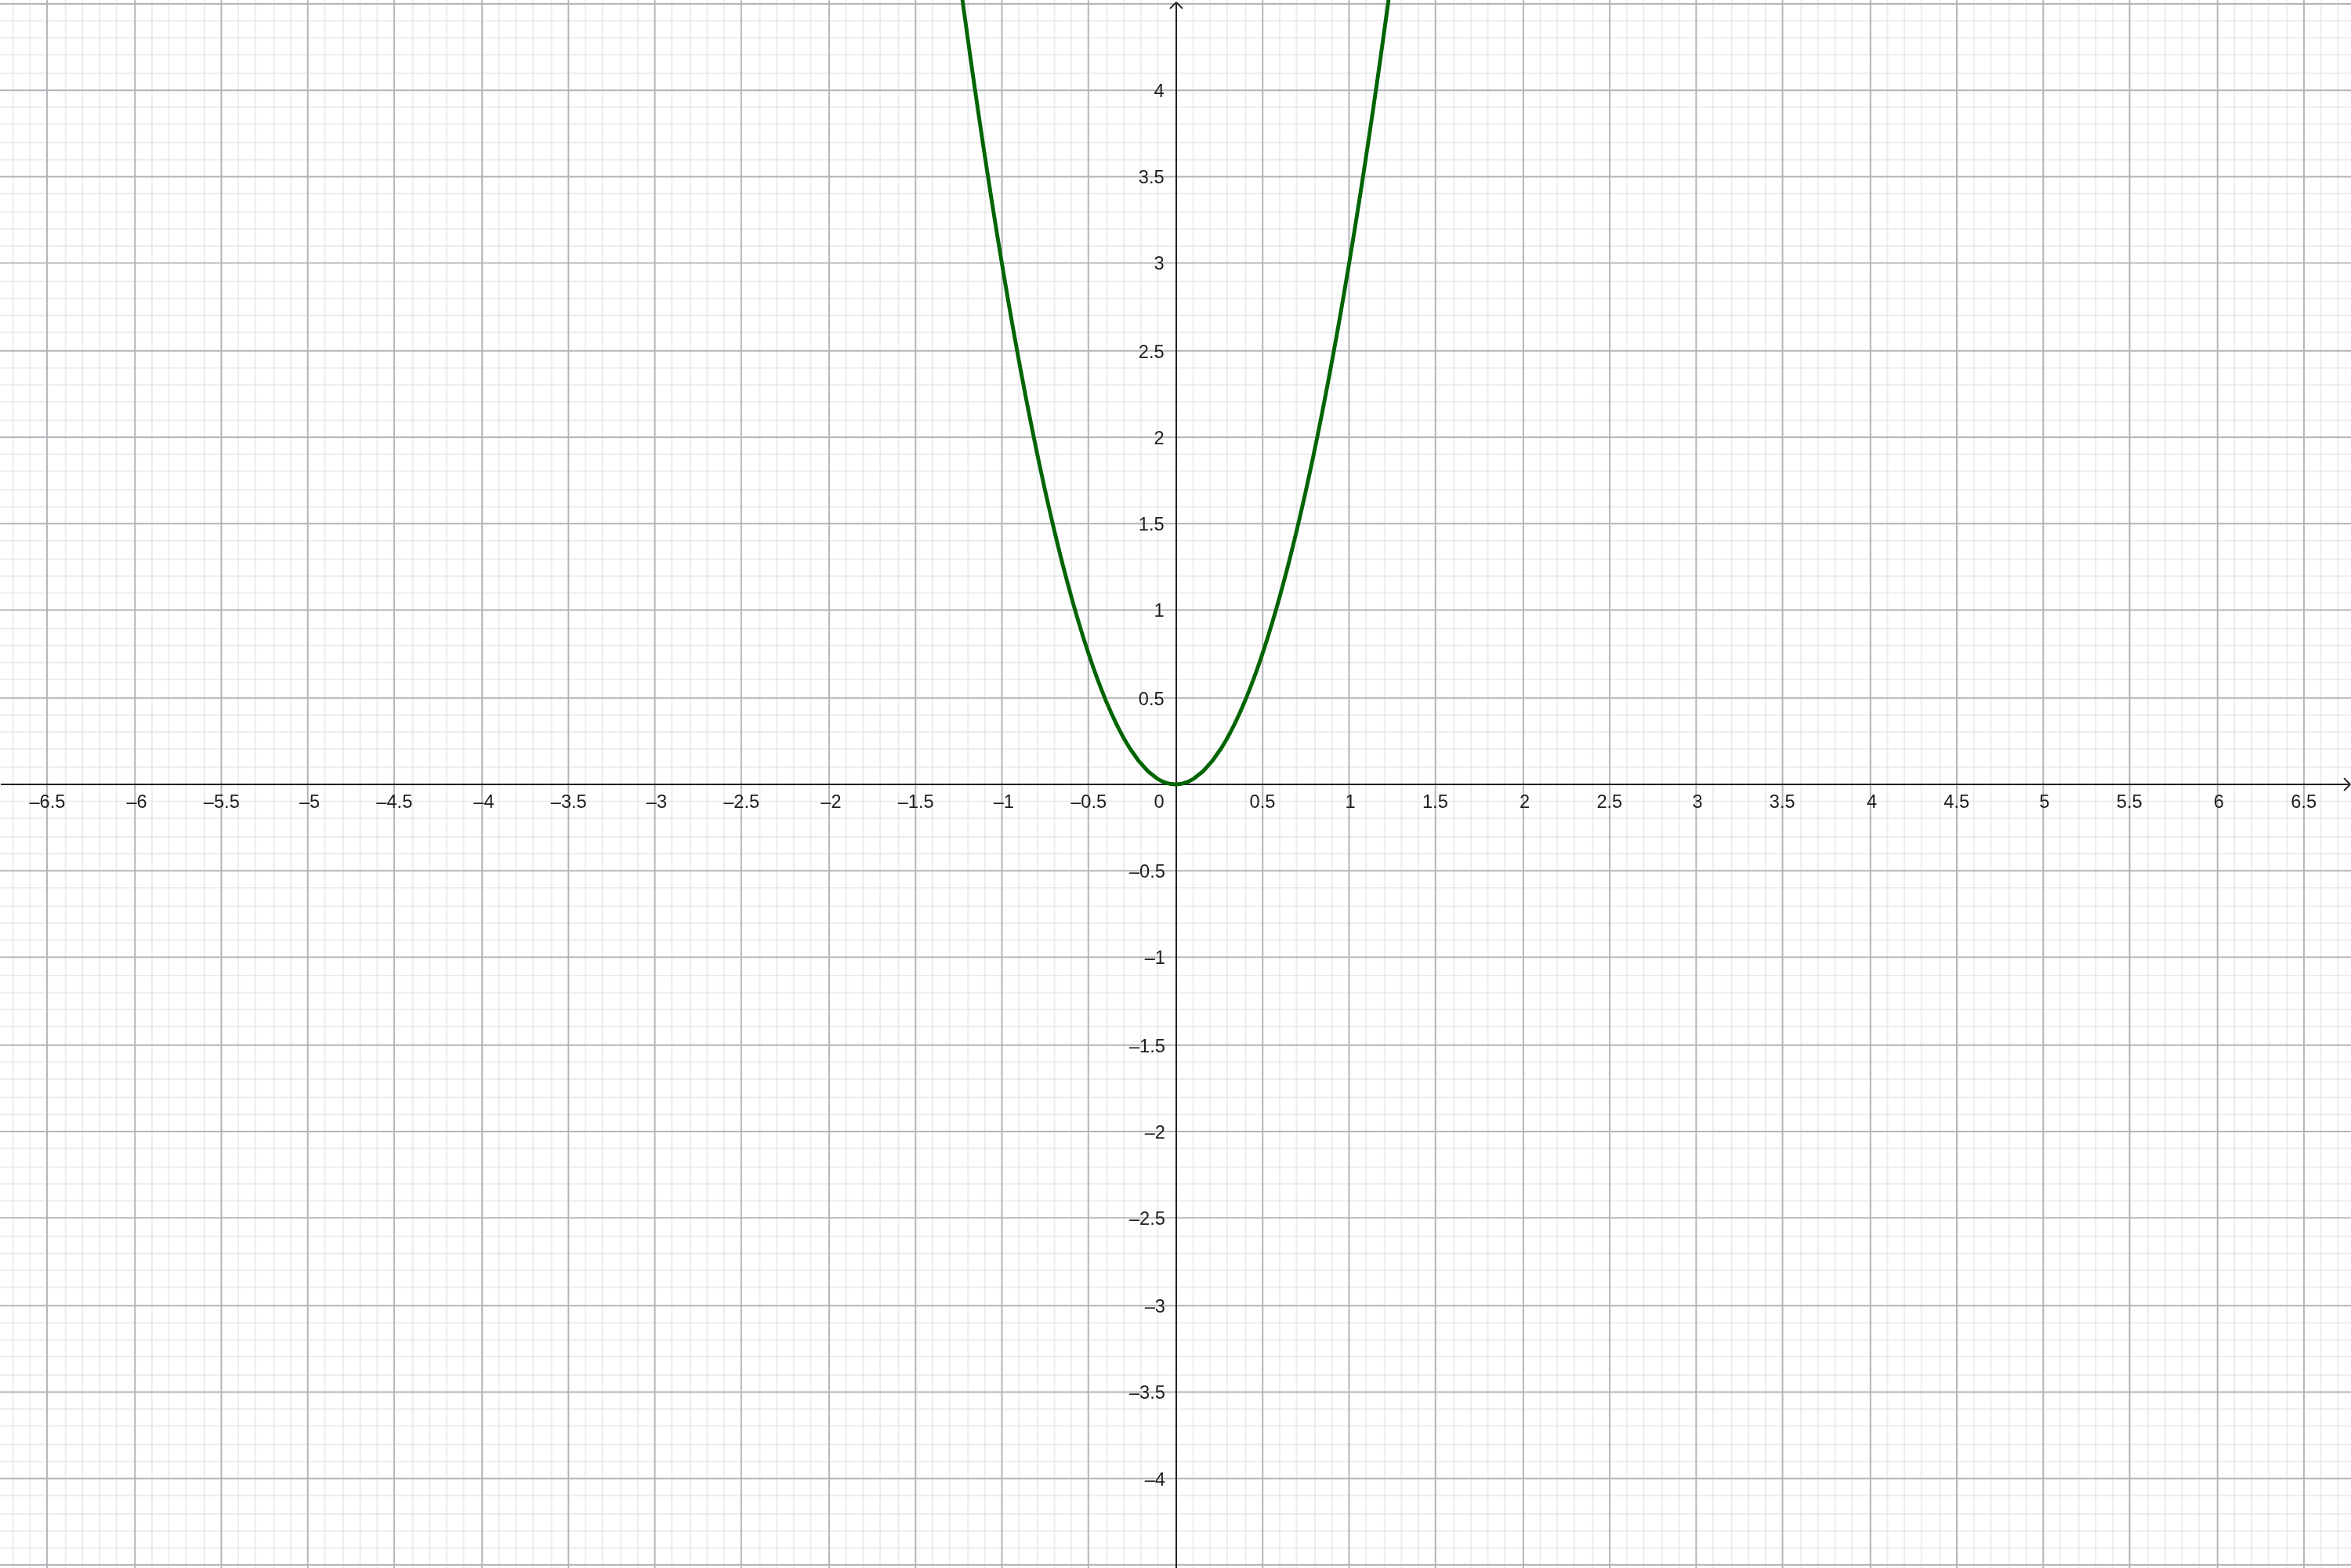
\includegraphics[width=0.7\linewidth]{./geogebra-export1.png}
\end{figure}
\newpage

% Actividad 2
\section*{Actividad 2}
\textbf{Instrucciones:} Encontrar $\frac{dy}{dx}$ si $x = t^2$ y $y = t^4$.
\newline

\textbf{Respuesta:}
\begin{align*}
	\frac{dy}{dt} &= 4t^3
\end{align*}
\begin{align*}
	\frac{dx}{dt} &= 2t
\end{align*}
\begin{align*}
	\frac{Dy}{dx} &= \frac{4t^3}{2t} \\
	&= \frac{4}{2} \cdot t^{3 - 1} \\
	&= 2t^2
\end{align*}

\begin{figure}[htb]
	\center
	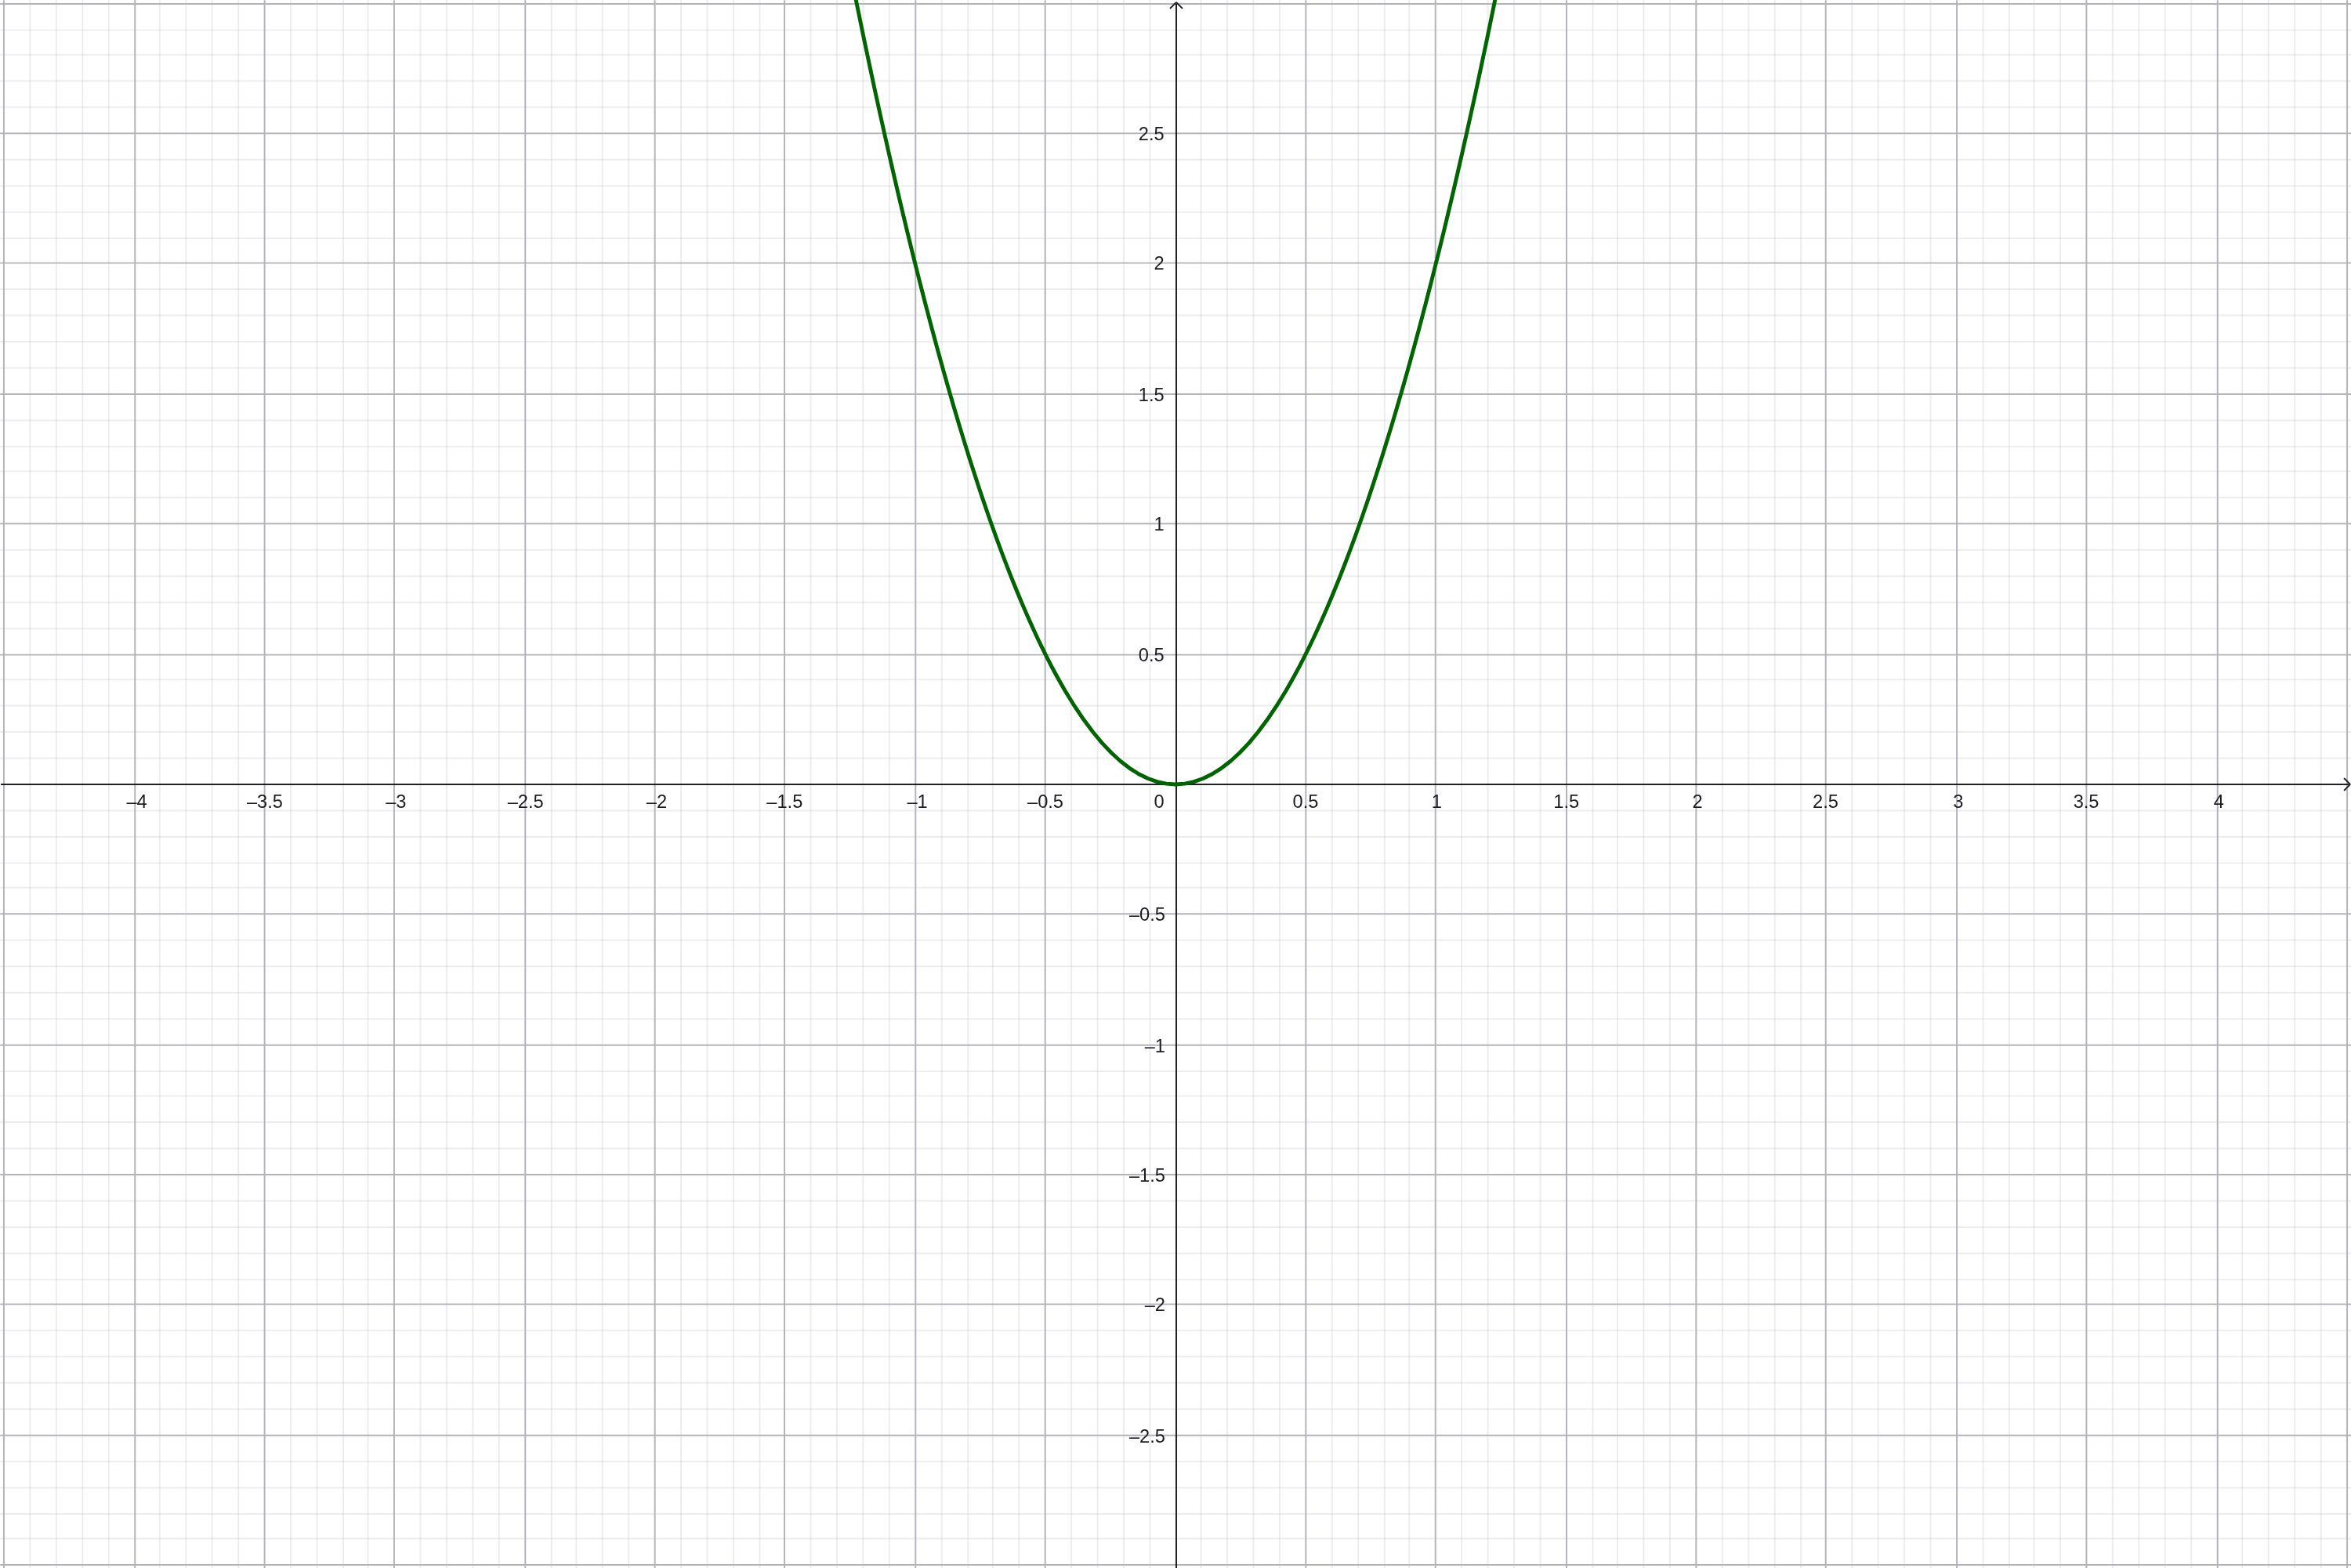
\includegraphics[width=0.7\linewidth]{./geogebra-export2.png}
\end{figure}
\newpage

% Actividad 3
\section*{Actividad 3}
\textbf{Instrucciones}: La trayectoria de un robot es $x = 3t$ y $y = t^2$. Determinar la pendiente cuando $t = 3$.
\newline

\textbf{Respuesta:}

\begin{align*}
	\frac{dy}{dt} &= 2t
\end{align*}
\begin{align*}
	\frac{dx}{dt} &= 3
\end{align*}
\begin{align*}
	\frac{Dy}{dx} &= \frac{2t}{3} \\
\end{align*}
\begin{align*}
	t &= 3 \\
	\frac{Dy}{dx} &= \frac{2(3)}{3} \\
	&= \frac{6}{3} \\
	&= 2
\end{align*}

\begin{figure}[htb]
	\center
	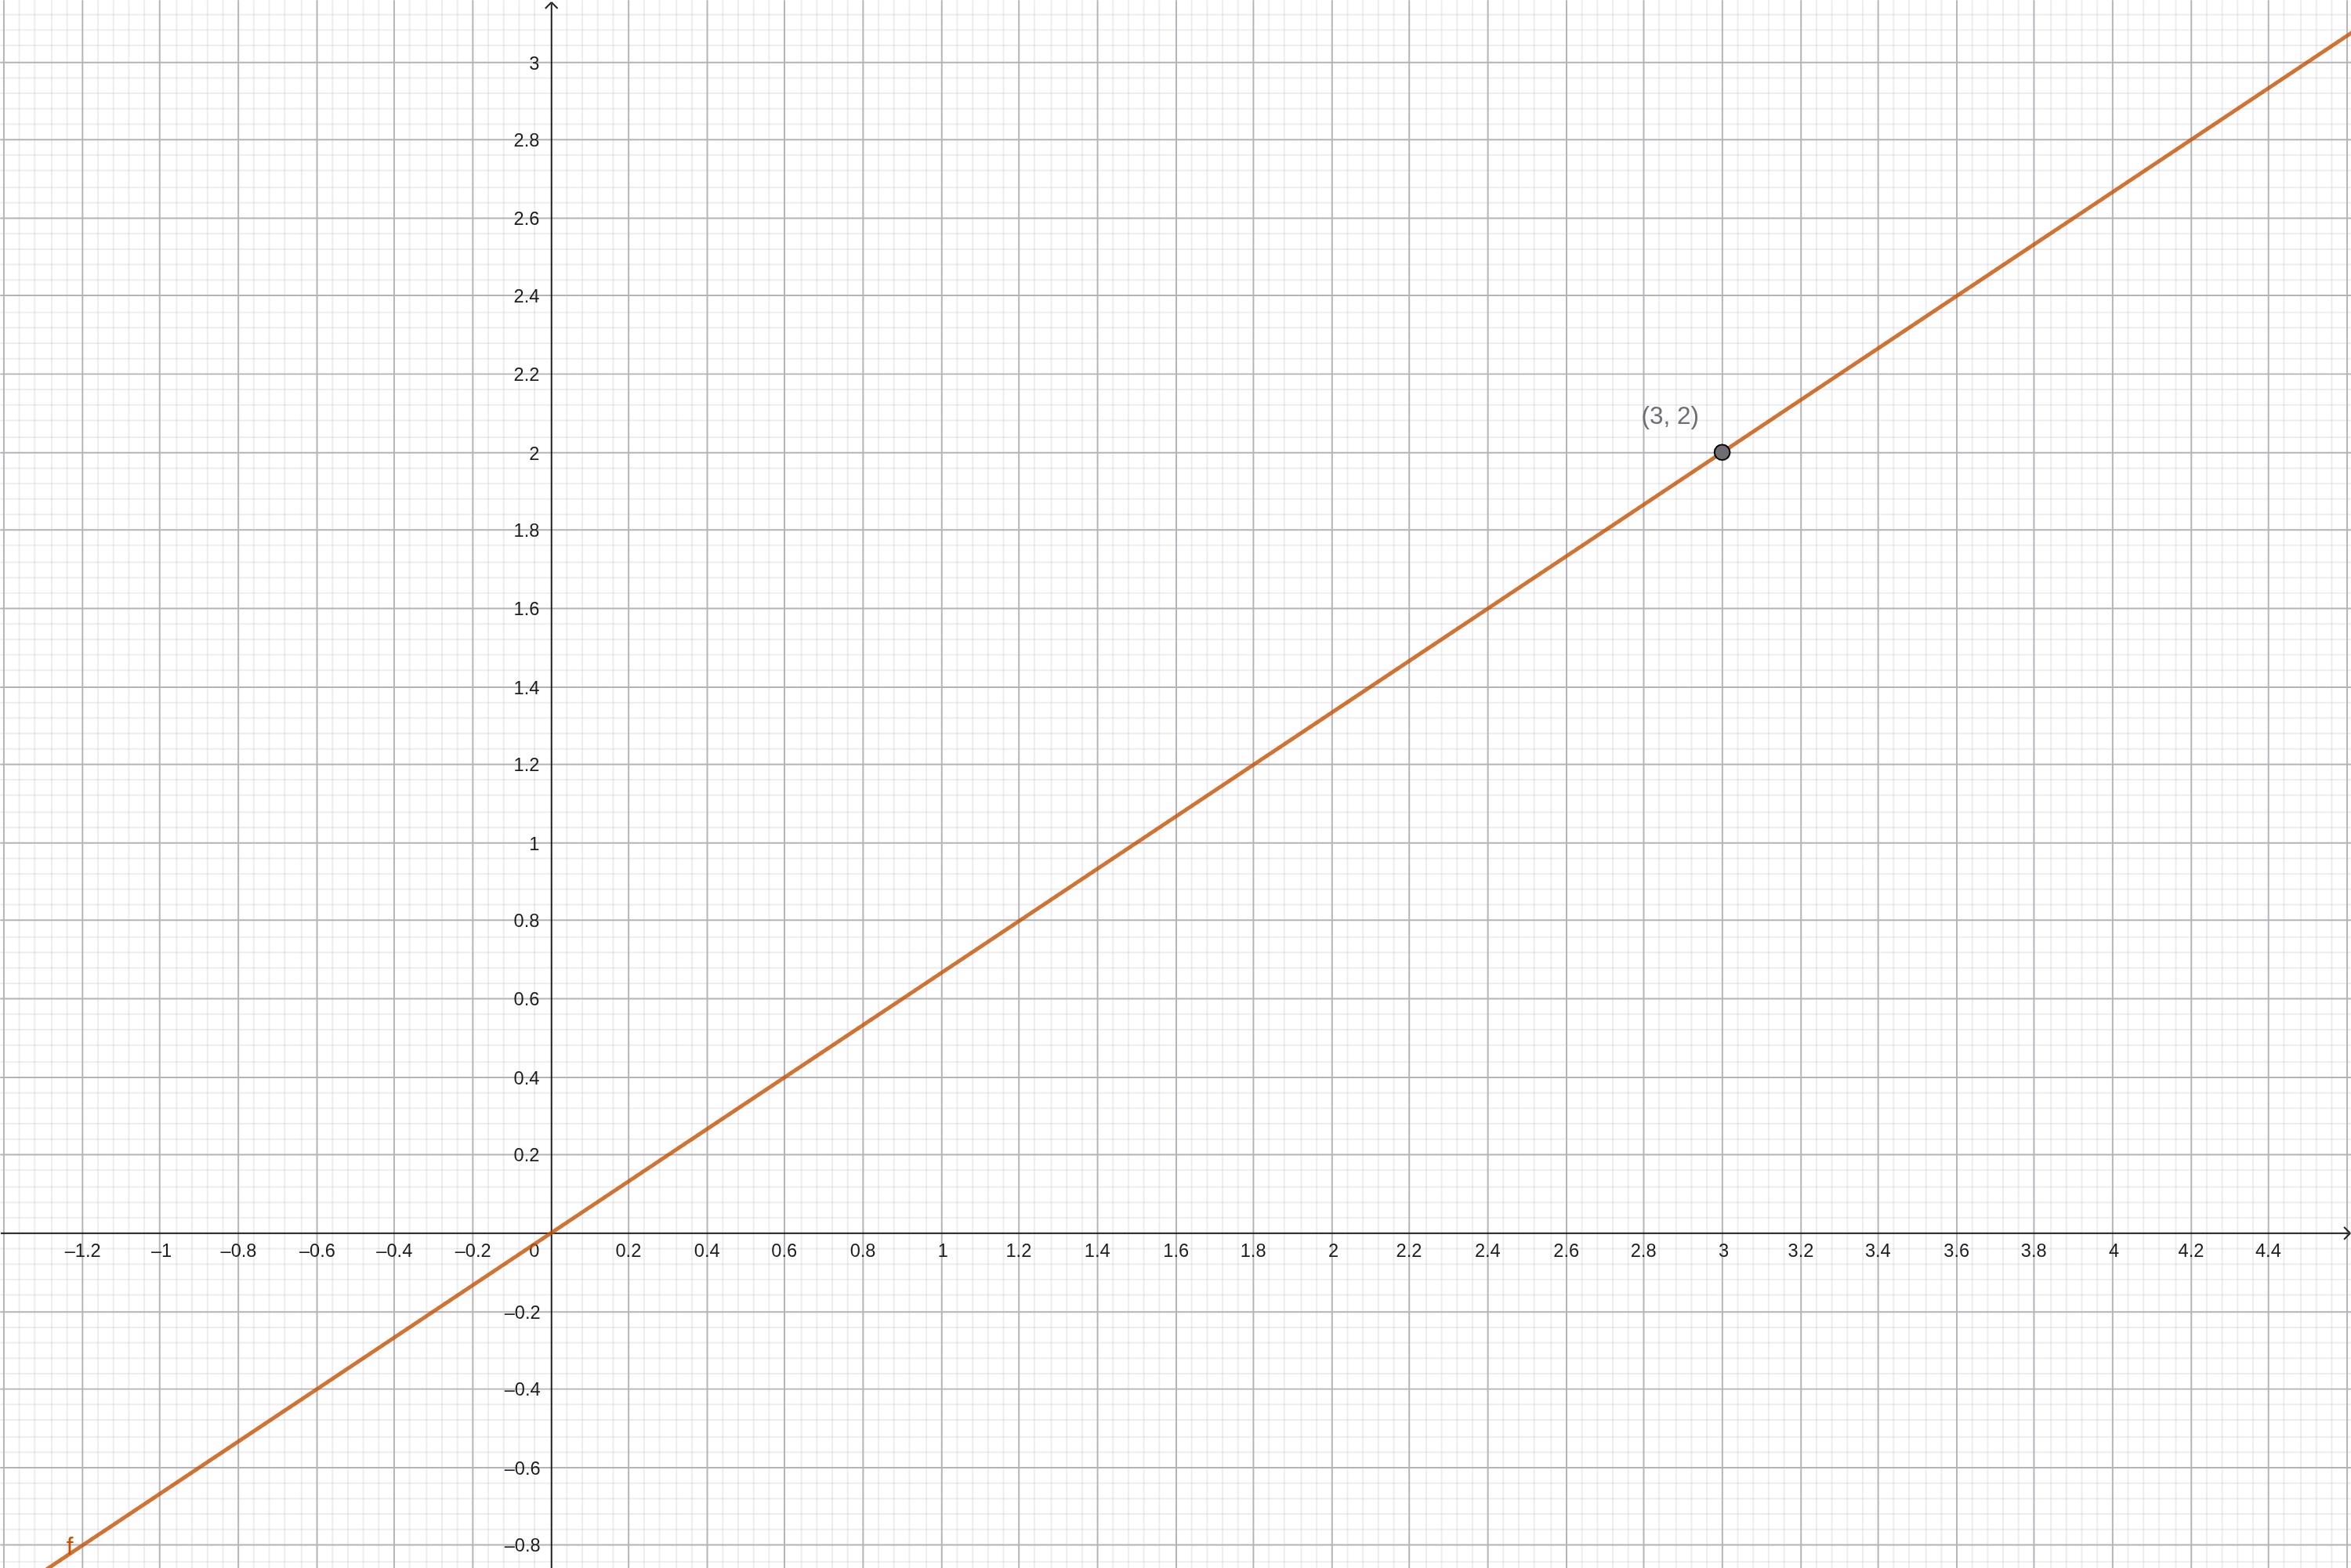
\includegraphics[width=0.7\linewidth]{./geogebra-export3.png}
\end{figure}

\end{document}
